%%%%%%%% ICML 2022 EXAMPLE LATEX SUBMISSION FILE %%%%%%%%%%%%%%%%%

\documentclass[nohyperref]{article}

% Recommended, but optional, packages for figures and better typesetting:
\usepackage{microtype}
\usepackage{graphicx}
\usepackage{subfigure}

\usepackage{booktabs} % for professional tables

% hyperref makes hyperlinks in the resulting PDF.
% If your build breaks (sometimes temporarily if a hyperlink spans a page)
% please comment out the following usepackage line and replace
% \usepackage{icml2022} with \usepackage[nohyperref]{icml2022} above.
\usepackage{hyperref}

\usepackage{graphicx}
\usepackage{subcaption}

% Attempt to make hyperref and algorithmic work together better:
\newcommand{\theHalgorithm}{\arabic{algorithm}}

% Use the following line for the initial blind version submitted for review:
% \usepackage{icml2022}

% If accepted, instead use the following line for the camera-ready submission:
\usepackage[accepted]{icml2022}

% For theorems and such
\usepackage{amsmath}
\usepackage{amssymb}
\usepackage{mathtools}
\usepackage{amsthm}


% if you use cleveref..
\usepackage[capitalize,noabbrev]{cleveref}

%%%%%%%%%%%%%%%%%%%%%%%%%%%%%%%%
% THEOREMS
%%%%%%%%%%%%%%%%%%%%%%%%%%%%%%%%
\theoremstyle{plain}
\newtheorem{theorem}{Theorem}[section]
\newtheorem{proposition}[theorem]{Proposition}
\newtheorem{lemma}[theorem]{Lemma}
\newtheorem{corollary}[theorem]{Corollary}
\theoremstyle{definition}
\newtheorem{definition}[theorem]{Definition}
\newtheorem{assumption}[theorem]{Assumption}
\theoremstyle{remark}
\newtheorem{remark}[theorem]{Remark}

% Todonotes is useful during development; simply uncomment the next line
%    and comment out the line below the next line to turn off comments
%\usepackage[disable,textsize=tiny]{todonotes}
\usepackage[textsize=tiny]{todonotes}


% The \icmltitle you define below is probably too long as a header.
% Therefore, a short form for the running title is supplied here:
\icmltitlerunning{\textsc{Latent-Mixup} : mixing latent variables to train robust classifiers}

\usepackage{caption}
\usepackage{subcaption}

\setcounter{secnumdepth}{5}
\setcounter{tocdepth}{5}

\makeatletter
\newcommand\subsubsubsection{\@startsection{paragraph}{4}{\z@}{-2.5ex\@plus -1ex \@minus -.25ex}{1.25ex \@plus .25ex}{\normalfont\normalsize\bfseries}}
\newcommand\subsubsubsubsection{\@startsection{subparagraph}{5}{\z@}{-2.5ex\@plus -1ex \@minus -.25ex}{1.25ex \@plus .25ex}{\normalfont\normalsize\bfseries}}
\makeatother


\begin{document}

\twocolumn[
\icmltitle{\textsc{Latent-Mixup} : mixing latent variables to train robust classifiers}

\begin{icmlauthorlist}
\icmlauthor{Tristan Girard}{}
\icmlauthor{Benjamin Gundersen}{}
\icmlauthor{Timothé Laborie}{}
\end{icmlauthorlist}

\vskip 0.3in
]

\begin{abstract}
In recent years there has been an impressive increase in the accuracy of Deep Neural Networks for classification such that for some specific tasks these networks achieve an accuracy above the average human level. At the same time, it has been shown that these networks are usually not robust to distribution shifts or adversarial attacks. A few years ago, the \textsc{Mixup} method was introduced. It involves training a model using convex combinations of training set inputs and their respective labels. This new method increases the model accuracy for some tasks and makes the models more robust. More recently that method has been generalized to mix the activations of the hidden layers inside a network, which lead to even more robust models. In our work we go one step further and do the mixing at the level of latent variables representing the images. We use both Generative Adversarial Networks (GAN) and Variational Auto-Encoders (VAE), we find the latent variables of the input images and train a standard classifier on images generated/decoded from a convex combination of the latent variables of the input images. We will briefly explain how \textsc{Mixup} and its generalization \textsc{Manifold Mixup} work. Building on these methods we then describe our approach. Finally, we show that training with our \textsc{GAN-Mixup} method yields more robust classifiers on certain datasets than training with \textsc{Manifold Mixup}.

\end{abstract}

\section{Introduction}

Current Deep Neural Network can be very accurate on the training set and still miss-classify with high confidence samples that slightly differ from the samples seen during training \cite{ben2010theory}, are underrepresented in the training set \cite{dro-hashimoto}, or are adversarial \cite{adv-szegedy}. Recently, the \textsc{Mixup} method has been proposed \cite{mixup1} and empirical evidence showed that classifiers trained with that method were more robust compared to models trained the standard way. The idea of \textsc{Mixup} is to augment the dataset with new images that are convex combinations of two images from the dataset. The label associated with the new image is the convex combination of the labels of the two original images with the same mixing factor. Generalizing that idea lead to \textsc{Manifold Mixup} where the hidden representations (activation of intermediate layers) inside a neural network are mixed instead of the raw samples. However, the challenge of developing fast training pipelines that also create robust models is still unsolved as even models trained with the methods above can be fooled with specific perturbations.

In order to increase the robustness even further we designed a training approach that builds on the \textsc{Mixup} idea but goes one step further. Instead of mixing the input features as in \textsc{Mixup} or the intermediate representations as in \textsc{Manifold Mixup}, we mix the latent codes of two samples that we got using a generative model. We then use that mixed latent code to generate a new sample that we associate with a label that is a convex combination of the original labels. Different generative models can be used in order to find the latent variables of images, we used GANs \cite{gan} which lead to the \textsc{GAN-Mixup} method and VAEs \cite{VAE} which lead to \textsc{VAE-Mixup}.

\subsection{\textsc{Mixup methods}}
In this section we will briefly describe the \textsc{Mixup} and \textsc{Manifold Mixup} methods, building on these algorithms we present \textsc{GAN-Mixup} and \textsc{VAE-Mixup} which mix the latent variables using different generative models. We tested our methods on the datasets MNIST, FashionMNIST and CIFAR-10.

\subsubsection{\textsc{Mixup}}
The \textsc{Mixup} training algorithm as presented in \cite{mixup1} is a data augmentation approach used in classification tasks. Pairs of samples are sampled from the dataset and a new data point is generated as a convex combination of the two original samples where the mixing factor $\lambda$ is drawn from a Beta distribution where the two parameters are set to $\alpha$ being a hyper-parameter. The mixed sample is then fed to the classification model which returns logits. The loss associated to that mixed sample is the convex combination of the loss of the logits with respect to the first label and the loss with respect to the second label, where the mixing factor is the same as the one used for the mixing of the inputs.

\subsubsection{\textsc{Manifold Mixup}}

Building on the \textsc{Mixup} idea the \textsc{Manifold Mixup} algorithm does not necessarily apply the mixing at the level of the inputs, instead a random hidden layer of the classification network is selected, two samples are sampled from the dataset and are fed to the classifier, for each sample we collect the activation of the selected hidden layer as a vector and then do the mixing over these activations vectors. The mixed activations are then fed to the layer coming directly after the selected layer and the network returns logits. The loss for the two samples is computed the same way as for the \textsc{Mixup} algorithm. If the input layer is selected to be the one where the representations are mixed, then that approach reduces to the standard \textsc{Mixup}. This is the reason why \textsc{Manifold Mixup} is a generalization of the former method.

\subsubsection{\textsc{Latent-Mixup}}
Numerical experiments done in the original paper show that training with \textsc{Mixup} yields models with a higher accuracy and which are more robust compared to models trained the standard way. In fact, very recent research shows that that training technique can be seen as a regularization technique \cite{mixup_reg}. The generalization \textsc{Manifold Mixup} performs better both in terms of accuracy and robustness \cite{mixup2}. It is well-know that the deeper a layer is, the more semantics its activation layers have \cite{visualizing}. Coupling that insight with the fact that mixing the representations works better on deeper layer than on the inputs lead to the idea that the mixing should be done on vectors containing an important share of the semantics of the image. Generative models such as GANs \cite{gan} and VAEs \cite{VAE} represent complex images in a low-dimensional space that summarises the most important aspects of the image. This inspired the decision to perform mixing on latent vectors of images instead of the inputs themselves or the activations of hidden layers. More specifically, we find latent vectors of the images in the training set and train a standard classifier on images generated/decoded from a convex combination of random pairs of latent vectors.

\section{Models and Methods}
\subsection{\textsc{GAN-Mixup}}
For each dataset, the \textsc{GAN-Mixup} process requires a GAN and a set of latent vectors that can accurately reconstruct the images from the training set.

\subsubsection{MNIST and FashionMNIST}
We train a GAN ourselves using a latent dimension of 1024. To invert the train set images, we use the methods described in \cite{ytLatentVector} which involves training an initializer model and a feature extractor. We optimize the initial latent vectors  using the L2 loss on the extracted visual features using 1000 gradient steps and AdamW \cite{ADAMW} with a learning rate of 0.03. After inverting the images, some of them had gotten stuck in a local minima due to a bad initialization, so we exclude the images where the reconstruction error is below average.

\subsubsubsection{\textsc{Training}}
For the classifier we use a generic convolution neural network with 575k parameters. When training each of the four methods described above, we use Adam \cite{ADAM} with 50 epochs, a learning rate of 0.001 and a learning rate decay of 0.9 per epoch.

\subsubsection{CIFAR-10}
As CIFAR-10 is a larger dataset than MNIST, we chose a StyleGAN2 model pre-trained on CIFAR-10 \cite{Karras2021}. This model has a FID of 2.384 on the CIFAR-10 dataset.

\subsubsubsection{StyleGAN Inversion}
To perform the inversion we employ the same approach as with the MNIST dataset, but this time in the W space of StyleGAN2.
The encoder is a copy of existing code from StyleGAN3-editing \cite{alaluf2022times} modified to work on the StyleGAN2 model that is pre-trained on CIFAR-10. After training different configurations we decided to use a ReStyle-pSp encoder using a ResNetBackBone, which was then trained for 5 days on a NVIDIA RTX 3090 GPU.

We then encode all 50-thousand training images and fine tune the latent vectors using gradient descent with the latent vectors as parameters and as loss a mixture ($\lambda_{LPIPS} = 0.9, \lambda_{L2} = 0.1$) between LPIPS \cite{lpips} and L2 of the original and reconstructed images. As optimizer we use AdamW with beta1 equal to $0.95$ and a learning rate of $0.03$. Using 1000 optimization steps, this takes about 30 seconds per image on a NVIDIA GeForce GTX 1080ti GPU. Doing this batched seemed to result in worse inversions, but it seems to be worthwhile to explore methods to do this batched without suffering from worse inversion. We ran this step on multiple GPUs in parallel. 


\begin{table*}[htbp]
\small
  \centering
  \begin{tabular}[c]{|l|l||l|l|l|}
    \hline
    Variant & Data Augmentation& Accuracy & DeepFool score & Blurred accuracy\\
    \hline
    Standard & None &0.8164 (0.0012) & 0.5322 (0.0297) & 0.3449 (0.0108) \\
    \textsc{Mixup} & None & 0.8416 (0.0038) & 0.5602 (0.0308) & 0.3623 (0.0098) \\
    \textsc{Manifold Mixup} & None & \textbf{0.8556 (0.0020)} & 0.6409 (0.0271) & 0.3759 (0.0046) \\
    \textsc{GAN-Mixup} & None & 0.8341 (0.0004) & 0.8675 (0.0269) & \textbf{0.4424 (0.0119)} \\
    \textsc{GAN-Mixup} (MSE $\geq$ 0.025) & None & 0.8326 (0.0059) & \textbf{0.9188 (0.0351)} & 0.4308 (0.0115) \\
    \textsc{GAN-Mixup} (MSE $\geq$ 0.020) & None & 0.8320 (0.0047) & 0.8701 (0.0968) & 0.4236 (0.0181) \\
    \hline
    \hline
    Standard & Random Flips + AutoAugment & \textbf{0.9139 (0.0005)} & 0.5327 (0.0171) & 0.4992 (0.0246) \\
    \textsc{Mixup} & Random Flips + AutoAugment & 0.9135 (0.0044) & 0.8514 (0.0355) & 0.4605 (0.0080) \\
    \textsc{Manifold Mixup}  & Random Flips + AutoAugment & \textbf{0.9139 (0.0035)} & 0.7107 (0.0224) & 0.4895 (0.0085) \\
    \textsc{GAN-Mixup} & Random Flips + AutoAugment & 0.8910 (0.0029) & 0.9576 (0.0022) & 0.5551 (0.0230) \\
    \textsc{GAN-Mixup} (MSE $\geq$0.025) & Random Flips + AutoAugment & 0.8875 (0.0045) & 0.9701 (0.0522) & 0.5557 (0.0198) \\
    \textsc{GAN-Mixup} (MSE $\geq$0.020) & Random Flips + AutoAugment & 0.8960 (0.0116) & \textbf{1.0213 (0.0404)} & \textbf{0.5581 (0.0270)} \\
    \hline
  \end{tabular}
  \caption{Results on the CIFAR-10 dataset}
  \label{tab:resultsc10}
\end{table*}

\subsubsubsection{Improving the latent vectors}\label{sec:improve_latent}

We additionally improve the worst latent vectors. First, we do an additional four thousand steps on the latent vectors which produce normalized images with a mean squared error (MSE) greater or equal to $0.025$ in comparison to the normalized original image. Then we do another 4000 steps with MSE greater or equal to $0.02$. The distributions of the MSE between normalized original and inverted images, as well as a few examples of the inversion process can be seen in Figures \ref{MSE1}, \ref{MSE2}, \ref{MSE3} and \ref{inv1}, \ref{inv2}, \ref{inv3} in the appendix.
The inverted images recover the original images with high fidelity.


\subsubsubsection{\textsc{Training}}
We use a ResNet18 \cite{resnet} as a classifier for all CIFAR-10 experiments. As optimizer we used SGD with 270 epochs, a batch size of 32 and an initial learning rate of 0.1 with ReduceLROnPlateau with a factor of 0.1.

\subsection{\textsc{VAE-Mixup}}
We trained a VAE the standard way on the dataset of interest using the standard loss. Once the VAE converged we augmented the dataset as follows: for random pairs of input images we got latent codes for the two images using the encoder network, we then did the mixing of the latent codes using some mixing factor $\lambda$, which lead to a unique latent code which we passed through the decoder network in order to get an image. This newly generated image is then sent to the classifier to get logits, the loss for that pair of image is then compute the same way as for \textsc{Mixup}. VAEs are known to generate blurry images, this is problematic as the images generated from the mixing of the latent codes were very blurry and thus negatively affected the accuracy of the trained classifier. One attempt to tackle that issue was to apply a sharpening filter to the images generated by the VAE.

\subsection{Training}
In order to find good hyperparameters for \textsc{VAE-Mixup} we ran a grid search and selected the hyperparameters with the highest validation accuracy.


\begin{table*}[htbp]
\small
  \centering
  \begin{tabular}[c]{|l||l|l|l|}
    \hline
    Variant & Accuracy & DeepFool score & Blurred accuracy\\
    \hline
    Standard & \textbf{0.9921 (0.0015)} & 1.4080 (0.0304) & \textbf{0.9343 (0.0115)} \\
    \textsc{Mixup} & 0.9884 (0.0031) & \textbf{4.0896 (0.0279)} & 0.6657 (0.0092) \\
    \textsc{Manifold Mixup} & 0.9886 (0.0025) & 3.8588 (0.0286) & 0.8429 (0.0046) \\
    \textsc{GAN-Mixup} & 0.9739 (0.0005) & 0.5328 (0.0271) & 0.7265 (0.0130) \\
    \hline
  \end{tabular}
  \caption{Results on the MNIST dataset}
  \label{tab:resultsmnist}
\end{table*}


\begin{table*}[htbp]
\small
  \centering
  \begin{tabular}[c]{|l||l|l|l|}
    \hline
    Variant & Accuracy & DeepFool score & Blurred accuracy\\
    \hline
    Standard & \textbf{0.9252 (0.0016)} & 0.3429 (0.0314) & 0.6727 (0.0123) \\
    \textsc{Mixup} & 0.8883 (0.0034) & \textbf{0.9098 (0.0216)} & 0.7163 (0.0087) \\
    \textsc{Manifold Mixup} & 0.9044 (0.0028) & 0.6736 (0.0265) & \textbf{0.7175} (0.0037) \\
    \textsc{GAN-Mixup} & 0.9192 (0.0014) & 0.3559 (0.0242) & 0.6769 (0.0135) \\
    \hline
  \end{tabular}
  \caption{Results on the FashionMNIST dataset}
  \label{tab:resultsfashionmnist}
\end{table*}



\section{Results}
We implemented our methods \textsc{GAN-Mixup} and \textsc{VAE-Mixup} using the PyTorch library \cite{pytorch}. We compare our methods with three different baselines. The first baseline is to simply train the classifier the standard way, the second baseline is \textsc{Mixup}, the third baseline is \textsc{Manifold Mixup}. For each variant we ran a grid-search on the hyperparameters and selected the ones yielding the highest classification accuracy on the validation set. We then reported the classification accuracy on the testing set as well as the DeepFool \cite{DeepFool} score and the accuracy on images blurred with a Gaussian kernel of size 5 from the testing set.

\textsc{VAE-Mixup} got an accuracy similar to the baselines, however the DeepFool scores and accuracy on the blurred images were much worse than the baselines on every dataset, thus the result section does not include the results of \textsc{VAE-Mixup}.

The training time of our method is significantly longer than for the other baselines as we have to find latent codes for the images and to generate a new image from the mixed latent codes. The main complexity overhead lies in that step. On the other hand, the inference is not affected at all as our method is a data augmentation technique which doesn't affect the architecture of the final classifier.

\subsection{\textsc{ CIFAR-10}}



We trained models using our method on the CIFAR-10 dataset as described in the previous section and reported the results with and without data augmentation. The data augmentation consists of random horizontal flips and the augmentation framework AutoAugment \cite{autoaug}. In addition to the standard \textsc{GAN-Mixup} we also included the results when we improved the worst latent codes as described in section \ref{sec:improve_latent}, these correspond to the entries \textsc{GAN-Mixup} (MSE $\geq$ 0.02) and \textsc{GAN-Mixup} (MSE $\geq$ 0.025) in the table showing the results.
The number in the parenthesis is the standard deviation over the different runs, we marked the best results with a bold font.
We can read from the result table \ref{tab:resultsc10} that \textsc{Manifold Mixup} yields the best classification accuracy both with and without data augmentation. Our method \textsc{GAN-Mixup} has an accuracy slightly lower than the \textsc{Manifold Mixup} but still outperforms the standard training without data augmentation in terms of accuracy. Looking at the robustness measures we see that \textsc{GAN-Mixup} outperforms the other variants both in terms of DeepFool score and accuracy on the blurred images. Training the classifier on a NVIDIA GeForce RTX 2080ti GPU takes about 30ms per batch for the standard method and 104ms for \textsc{GAN-Mixup}.


\subsection{MNIST and FashionMNIST}

We trained models using our method on the MNIST and FashionMNIST datasets as described in the previous sections. On FashionMNIST, we set it up so that half of the data comes from original images, as we found it improves all of the metrics.
We can read from the result table \ref{tab:resultsmnist} that the standard training procedure yields the best classification accuracy. Our method \textsc{GAN-Mixup} did not improve the robustness on either dataset compared to \textsc{Manifold-Mixup}, but it does get a better accuracy than both other Mixup methods on FashionMNIST. Looking at the robustness measures we see that \textsc{Mixup} outperforms the other variants in terms of DeepFool score.

\section{Discussion}
In this research, we present a method for improving the adversarial robustness of a classifier using GAN and VAE interpolation. Our experiments show that the GAN-Mixup method was effective on the CIFAR-10 dataset, where it is able to significantly improve the classifier's robustness against adversarial attacks as measured by DeepFool, while keeping the accuracy comparable or a bit lower than the standard training procedure. However, when we tried to apply a similar method on the MNIST and FashionMNIST datasets, we did not see the same improvement.

One possible explanation for this difference in performance is that the StyleGAN2 model trained on CIFAR-10 is a lot more complex and fits the data distribution closer. The StyleGAN2 model we used has a FID of 2.384. 
Another explanation is that we spent far more computational resources to invert the CIFAR-10 GAN and retrieve the latent vectors. 
It might also be the case that the StyleGAN2 latent space is more well behaved for interpolation. When we plotted some interpolated images from the MNIST GAN, most of them just looked like one of the original labels.

The VAE-Mixup method performed worse in every situation. This may be because the VAEs that we used have a much lower model complexity than StyleGAN2.

Overall, our results suggest that GAN interpolation is a promising method for improving adversarial robustness, but more work is needed to understand its limitations and to explore other ways of improving the robustness of classifiers to adversarial attacks.


\section{Summary}
Our experiments show that the GAN interpolation method was effective on the CIFAR-10 dataset. From this, we conclude that \textsc{GAN-Mixup} is a promising method to improve robustness. This method is computationally demanding and so is the inversion. Implementing and comparing different methods of inversion is a time consuming endeavour.

In conclusion, \textsc{GAN-Mixup} is a promising method to provide robustness against adversarial attacks and potentially improves the accuracy if the latent vectors are of high quality. This improvement comes with a cost in computational time, complexity of code and the time needed to compare and come up with ways on how to invert the images.

\bibliography{bibliography}
\bibliographystyle{icml2022}

\newpage
\appendix
\onecolumn

\section{MSE of latent vectors}
\begin{figure}[ht]
\begin{center}
    \includegraphics[width=0.8\textwidth]{plots/MSEnoopt.png}
    \caption{MSE of latent vectors, no additional steps}
    \label{MSE1}
\end{center}
\end{figure}


\begin{figure}[ht]
\begin{center}
    \includegraphics[width=0.8\textwidth]{plots/MSE0.025.png}
    \caption{MSE of latent vectors, additional steps for $0.025$}
    \label{MSE2}
\end{center}
\end{figure}

\begin{figure}[ht]
\begin{center}
    \includegraphics[width=0.8\textwidth]{plots/MSE0.02.png}
    \caption{MSE of latent vectors, additional steps for $0.02$}
    \label{MSE3}
\end{center}
\end{figure}

\clearpage
\section{CIFAR-10 Inversion Examples}
\begin{figure}[ht]
    \centering
    \begin{subfigure}{ }
        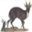
\includegraphics[width=0.12\textwidth]{inversion_images/original_04503_4.png}
    \end{subfigure}
    \begin{subfigure}{ }
        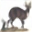
\includegraphics[width=0.12\textwidth]{inversion_images/inversion_04503_4.png}
    \end{subfigure}
    \begin{subfigure}{ }
        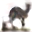
\includegraphics[width=0.12\textwidth]{inversion_images/encoder_04503_4.png}
    \end{subfigure}
    \caption{original image (left), inverted image (center), encoded image (right)}
    \label{inv1}
\end{figure}

\begin{figure}[ht]
    \centering
    \begin{subfigure}{ }
        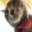
\includegraphics[width=0.12\textwidth]{inversion_images/original_17243_3.png}
    \end{subfigure}
    \begin{subfigure}{ }
        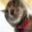
\includegraphics[width=0.12\textwidth]{inversion_images/inversion_17243_3.png}
    \end{subfigure}
    \begin{subfigure}{ }
        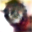
\includegraphics[width=0.12\textwidth]{inversion_images/encoder_17243_3.png}
    \end{subfigure}
    \caption{original image (left), inverted image (center), encoded image (right)}
    \label{inv2}
\end{figure}

\begin{figure}[ht]
    \centering
    \begin{subfigure}{ }
        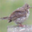
\includegraphics[width=0.12\textwidth]{inversion_images/original_43421_2.png}
    \end{subfigure}
    \begin{subfigure}{ }
        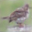
\includegraphics[width=0.12\textwidth]{inversion_images/inversion_43421_2.png}
    \end{subfigure}
    \begin{subfigure}{ }
        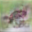
\includegraphics[width=0.12\textwidth]{inversion_images/encoder_43421_2.png}
    \end{subfigure}
    \caption{original image (left), inverted image (center), encoded image (right)}
    \label{inv3}
\end{figure}

\iffalse

\section{Experimental results}
Maybe put some stuff from the main report here


\begin{table*}[htbp]
\small
  \centering
  \begin{tabular}[c]{|l||l|l|l|}
    \hline
    Variant & Accuracy & DeepFool score & Blurred accuracy\\
    \hline
    Standard & 0.8164 (0.0012) & 0.5322 (0.0297) & 0.3449 (0.0108) \\
    Mixup & 0.8416 (0.0038) & 0.5602 (0.0308) & 0.3623 (0.0098) \\
    Manifold & 0.8556 (0.0020) & 0.6409 (0.0271) & 0.3759 (0.0046) \\
    GAN & 0.8341 (0.0004) & 0.8675 (0.0269) & 0.4424 (0.0119) \\
    VAE & 0.9139 (0.0005) & 0.5327 (0.0171) & 0.4992 (0.0246)\\
    \hline
  \end{tabular}
  \caption{MNIST results}
  \label{tab:results}
\end{table*}

\begin{center}
\begin{tabular}{ c c c c c c c}
variant & mean accuracy & std accuracy & mean deepfool & std deepfool & blurred acc & blurred std\\
standard & $0.8164$ & $0.0012$ & $0.5322$ & $0.0297$ & $0.3449$ & $0.0108$ \\
mixup & $0.8416$ & $0.0038$ & $0.5602$ & $0.0308$ & $0.3623$ & $0.0098$ \\
manifold & $0.8556$ & $0.0020$ & $0.6409$ & $0.0271$ & $0.3759$ & $0.0046$ \\
GAN & $0.8341$ & $0.0004$ & $0.8675$ & $0.0269$ & $0.4424$ & $0.0119$ \\
VAE & $0.9139$ & $0.0005$ & $0.5327$ & $0.0171$ & $0.4992$ & $0.0246$\\
\end{tabular}
\end{center}
\fi



\end{document}
